\documentclass{article}
\usepackage{tikz}
\usepackage{hyperref}
\usepackage{xcolor}

\hypersetup{
  colorlinks=true
}

\usetikzlibrary{intersections}

\title{On sailing forces}
\begin{document}
\maketitle
This is a simplified graph of the forces that make a boat sail windward. I am
assuming that there is no hydrodynamic drag here, and that the apparent speed of
the water is parallel to the direction of the boat. Otherwise, the keel also
acts as a wing with respect to water, generating lift and drag, which decompose
to a side force and a force opposing to the driving force, thus ending up on the
boat moving sideways and a reduced total force pushing the boat forward.

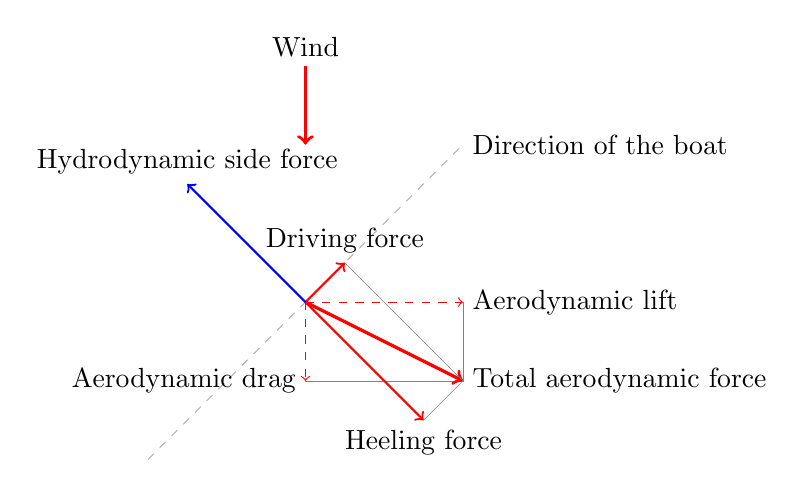
\begin{tikzpicture}
  % Boat
  \draw[help lines, dashed] (-2,-2) -- (2,2);
  \node[above, right] at (2,2) {Direction of the boat};

  % Wind
  \draw[very thick, red, ->] (0,3) -- (0,2);
  \node[above] at (0,3) {Wind};

  % Aerodynamic forces
  \draw[red, dashed, ->] (0,0) -- (2,0);
  \node[right] at (2, 0) {Aerodynamic lift};

  \draw[red, dashed, ->] (0,0) -- (0, -1);
  \node[below, left] at (0, -1) {Aerodynamic drag};

  \draw[help lines] (0, -1) -- (2, -1) -- (2, 0);
  \draw[very thick, red, ->] (0,0) -- (2, -1);
  \node[below, right] at (2, -1) {Total aerodynamic force};

  \draw[red, thick, ->] (0,0) -- (intersection cs:
  first line={(0,0) -- (3, 3)},
  second line={(2, -1) -- (1, 0)}) coordinate (Fr);
  \node[right, above] at (Fr) {Driving force};

  \draw[red, thick, ->] (0,0) -- (intersection cs:
  first line={(0,0) -- (3, -3)},
  second line={(2, -1) -- (1, -2)}) coordinate (Fh);

  \draw[help lines] (Fr) -- (2, -1) -- (Fh);
  \node[below] at (Fh) {Heeling force};

  % hydrodynamic forces
  \draw[thick, blue, ->] (0,0) -- (intersection cs:
  first line={(0,0) -- (-1, 1)},
  second line={(-2, 1) -- (-1, 2)}) coordinate (Fs);
  \node[above] at (Fs) {Hydrodynamic side force};
\end{tikzpicture}

Nice summary of the forces involved
\href{http://grizzly.colorado.edu/~rmw/files/papers/PhysicsofSailing.pdf}{here}.

\begin{itemize}
\item The aerodynamic lift force (\overrightarrow{L}) is perpendicular to the
  wind.
\item The aerodynamic drag force (\overrightarrow{D}) goes in the direction of
  the wind.
\item The total aerodynamic force is the sum of lift and drag
  $\overrightarrow{F}_T = \overrightarrow{L} + \overrightarrow{D}$.
\item The driving force ($\overrightarrow{F}_R$) goes parallel to the point of
  sail.
\item The heeling force ($\overrightarrow{F}_H$) goes perpendicular to the point
  of sail.
\item Hydrodynamic side force ($\overrightarrow{F}_S$) is the ``lift'' generated
  by the keel against the water. It goes perpendicular to the apparent motion of
  water.
\item The hydrodynamic drag force (\overrightarrow{D}) goes parallel to the
  keel.
\item The total hydrodynamic force is $\overrightarrow{R}_T =
  \overrightarrow{F}_S + \overrightarrow{R}$.
\end{itemize}

We assume that lift and drage are generated somehow by the sail. The actual
physics of how this happens are quite complex. A sail that has a small angle to
the wind generates less drag, but also less lift. Play with
\href{https://www.grc.nasa.gov/www/k-12/airplane/foil3.html}{foil simulator}, to
experiment.

In the chart, the sail generates a total aerodynamic force that we decompose in
lift and drag to illustrate how both forces interact, but is not necessary to do
this to understand how the sail pushes the boat. Is just necessary that the
total aerodynamic force has an angle with the direction of the boat that is
smaller than 90 degrees (so that there is a driving force component). To see how
the total aerodynamic force moves the boat, we assume that it is not possible to
push the boat out of the sailing line, and decompose the total aerodynamic force
into the heeling force and driving force components. The heeling force is
compensated by the hydrodynamic side force, but the residual driving force
accelerates the boat.
\end{document}
